% !TEX root = ./report.tex

\clearpage
\section{The Inliner}
\label{scheme:start}

\thiswillnotshow[inline]{Introduce section with how the RVSDG helps with the different
steps in the below enumerated list.}

The following heuristic is executed by the inliner of this project when given an
RVSDG as input:

\begin{enumerate}
	\item For all recursive environments ($\phi$-regions):

	\begin{enumerate}
		\item Use the approach described in
Section~\ref{sub:scheme:inlining_recur_apply_nodes} to fill a list of
\textit{loop breakers}. These $\lambda$-nodes are \textit{not} to be inlined.
		\label{MakeLoopBreakerListItem}
	\end{enumerate}

	\item Scan through the RVSDG, finding all \applyNode s. Exclude all function
calls to loop breakers, calls invoking functions that are not-statically known,
or external functions.
	\label{ScanForApplyNodesItem}

	\item Make a list of the \applyNode s found in
Step~\ref{ScanForApplyNodesItem}, and order the list of according to the
heuristics discussed in Section~\ref{sub:scheme:ordering_apply_nodes}.
The order of \applyNode s inlined can affect the amount of \applyNode s inlined,
even when each \applyNode~is evaluated with the same heuristic.
	\label{OrderApplyNodesFoundItem}

	\item Look at each \applyNode~in turn from the list made in
Step~\ref{OrderApplyNodesFoundItem} and decide whether or not to inline it
according to the heuristic discussed in \ref{sub:scheme:inlining_apply_nodes}:
	\label{LookAtNextCallSiteItem}

	\begin{enumerate}
		\item If the \applyNode~is inlined, add any newly copied (inlined)
\applyNode s, following the same criteria as used in
Step~\ref{ScanForApplyNodesItem}, to the list of \applyNode s. Continue with
Step~\ref{OrderApplyNodesFoundItem}.

		\item If the \applyNode~is not inlined, continue with
Step~\ref{LookAtNextCallSiteItem}, evaluating the next \applyNode .
		\label{InlineCallSiteItem}
	\end{enumerate}

	\item When the inliner reaches the end of the list, no more \applyNode s
have been inlined, and the inliner is finished.
\end{enumerate}

\subsection{Deciding which recursive functions to inline}
\label{sub:scheme:inlining_recur_apply_nodes}

The inliner evaluates all functions, recursive or not, with the same heuristic,
described in Section~\ref{sub:scheme:inlining_apply_nodes}. However, the inliner
of this project only evaluates \textit{some} of the \applyNode s invoking
recursive functions, to ensure termination of the compiler.

The \applyNode s not evaluated for inlining are the \textit{loop breakers},
found in Step~\ref{ScanForApplyNodesItem}. Loop breakers are function-nodes
found in $\phi$-regions which are self-recursive, and function-nodes which break
Strongly Connected Component cycles within the $\phi$-region's call dependency
graph.

\todo[inline]{Make a figure or three of $phi$-regions, one with a self-recursive
lambda, one with some mutually recursive ones (the example from PVV w/Torje),
and perhaps also one based on GHC papers FGHPQ example.}

Hence, the inliner has a list of recursive functions which it knows \textit{not}
to inline, thus ensuring termination of the compilation. All other remaining
recursive functions may then be safely inlined with the same criteria as any
non-recursive functions.

\subsection{The order of call sites inlined}
\label{sub:scheme:ordering_apply_nodes}

\todo[inline]{Need reference to further ideas section related to ordering of
inlining, when finished.}

The heuristic deciding on whether or not to inline a specific \applyNode~is
based on previous work; Keith D. Cooper et. al~\cite{AdaptvStratInlSubst} and
Waterman~\cite{AdaptvCompilAndInlingWaterman}. Their work utilizes
\textit{Inlining Conditions}\footnote{Introduced in
Section~\ref{sub:meth:inlining_conditions}.} (ICs), which evaluate properties of
the function invoked or the call-site(s) invoking said function. As such, when a
successive series of functions call one another, our approach only considers one
function's properties or \applyNode (s)'s properties, at a time.

\info[inline]{Because of above paragraph, which I think belongs to
Section~\ref{sub:scheme:inlining_apply_nodes}, ask Nico if he insists that
Section~\ref{sub:scheme:ordering_apply_nodes} should come before
Section~\ref{sub:scheme:inlining_apply_nodes}. I feel that this makes little
sense since the one that is first now relies on the second...}

Hence, for some ICs such as \textit{Statement Count} it makes a difference which
order the \applyNode s are evaluated in, as shown in
Figure~\ref{fig:inline_ordering_ex}. If our criteria for inlining is that the
function being inlined does not exceed the IC ``SC $> 4$'', and the \applyNode s
in dependency call graph depicted in Figure~\ref{fig:inline_ordering_ex} are
evaluated top-down, $\lambda_1$ can be inlined into $\lambda_2$. The new
$\lambda_{1-2}$ can be inlined into $\lambda_3$, resulting in all of them being
inlined into a single function $\lambda_{1-2-3}$.

\begin{figure}[H]
	\centering
	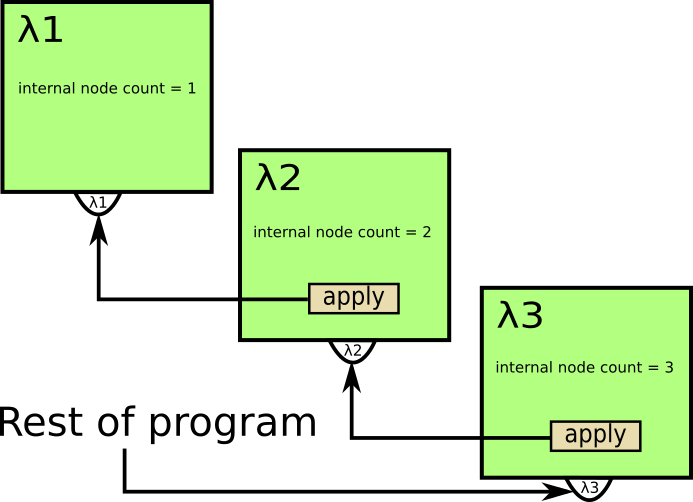
\includegraphics[width=0.75\textwidth]{figures/inline_ordering_ex}
	\caption{A minimal example of an RVSDG subgraph, depicting a function call
order in a program.}
	\label{fig:inline_ordering_ex}
\end{figure}

However, if the \applyNode s are evaluated in the opposite order, bottom-up with
the same inlining requirement, $\lambda_3$ can be inlined into $\lambda_2$, but
$\lambda_{2-3}$ cannot be inlined into $\lambda_1$. Thus, the amount of
\applyNode s inlined differ for the same dependency call graph, when the only
variable is the order the \applyNode s are evaluated in.

\subsection{Inlining a call site}
\label{sub:scheme:inlining_apply_nodes}

Our approach was chosen because it permits effective testing for an apt
heuristic when deciding on whether or not to inline a call site.

As mentioned, the inliner uses several different ICs: SC, \textit{Static Call
Count} (SCC), and \textit{Loop Nesting Depth} (LND) being among these. These ICs
and others described in Section~\ref{sub:meth:inlining_conditions}, allow us to
write and re-write the inlining heuristic effectively, since we can write them
using \textit{Conjunctive Normal Form} (CNF) in the following fashion:
\lstinline"SC < X || SCC < Y || (SCC < Z && LND > W)".

This allows us to efficiently search the parameter space for optimal parameters
for the inlining heuristics.

\todo[inline]{Describe the algorithm and inliner conditions we land for
evaluating a call site on after testing.}
